\section{Auswertung}
\label{sec:Auswertung}
\subsection{Theoretische Werte}
\label{subsec:theoW}
Es werden die drei Stoffe Neodym, Gadolinium und Dysprosium untersucht. Um die theoretischen Werte der magnetischen Suszeptibilität $\chi$ berechnen zu können, müssen zunächst die Quantenzahlen bestimmt werden.
Dafür muss auf den Aufbau der drei Proben eingegangen werden. Die Werte sind in \autoref{tab:quantZahl} zusammengefasst.
Alle Stoffe sind Metalle der Seltenen Erden und haben damit eine komplette 5p-Schale und 2s-Elektronen, die aber für den Paramagnetismus unwichtig sind, da die Spins und Bahndrehimpulse abgesättigt sind
und der resultierende Drehimpuls verschwindet. Da die Seltenen Erd Metalle alle ein 4f-Elektron mehr haben, als ihre Vorgänger, folgen die Anzahl der 4f-Elektronen jeweils für die drei Stoffe.
Somit hat Neodym 4 Elektronen, Gadolinium hat 8  und Dysprosium hat dementsprechend 10 Elektronen auf der 4f-Schale.
Wenn ein Atom Ionisiert wird, verliert es ein 6s- und ein 4f-Elektron.
Gemäß der Hund'schen Regeln werden die Quantenzahlen berechnet.
Der Landé-Faktor $g_j$ wird nach Gleichung (\ref{eqn:landeF}) berechnet.

\begin{table}[H]
  \centering
  \caption{Bestimmung der Quantenzahlen.}
  \label{tab:quantZahl}
  \begin{tabular}{c| c c c c c c}
    \toprule
    Element & $4f_{\text{neutral}}$ & $4f_{\text{ionisiert}}$ & S & L & J & $g_j$\\
    \midrule
    Neodym & 4 & 3 & $3\cdot\sfrac{1}{2}=\sfrac{3}{2}$ & 6 & $\sfrac{9}{2}$ & 0.727 \\
    Gadolinium & 8 & 7 & $7\cdot\sfrac{1}{2}=\sfrac{7}{2}$ & 0 & $\sfrac{7}{2}$ & 2 \\
    Dysprosium & 10 & 9 & $7\cdot\sfrac{1}{2}-2\sfrac{1}{2}=\sfrac{5}{2}$ & 5 & $\sfrac{15}{2}$ & 1,382 \\
    \bottomrule
  \end{tabular}
\end{table}

\noindent
Für die theoretische Suszeptibilität $\chi$ wird noch de Anzahl $N$ der der atomaren magnetischen Dipolmomente pro Volumeneinheit benötigt, der mithilfe der Gleichung 
\begin{align*}
  N = \frac{\rho}{m_{\text{mol}}} = \frac{\rho}{V_{\text{mol}} \cdot \rho} = \frac{1}{V_{\text{mol}}} %Masse *10**(-3) / (Volumenmol * 10**(-6) * u)
\end{align*}
berechnet wird.
In \autoref{tab:abmProben} sind die Volumina pro Mol und die atomaren, magnetischen Dipolmomente der drei in dem Versuch verwendeten Proben zu entnehmen.
\begin{table}[H]
  \centering
  \caption{Abmaße der drei Proben.}
  \label{tab:abmProben}
  \begin{tabular}{c|c c}
    \toprule
    Stoff & $V_{\text{mol}}$ \,/\, $\si{\micro\cubic\meter\per\mole}$ & $N$ \,/\, $\sfrac{10^{29}}{\si{\cubic\meter}}$ \\
    \midrule
    Neodym & 20,59 & 5,405 \\
    Gadolinium & 19,90 & 4,261 \\
    Dysprosium & 19,01 & 4,754 \\
    \bottomrule
  \end{tabular}
\end{table}

\noindent
Die magnetische Suszeptibilität ist von der Temperatur abhängig. Der Versuch wurde bei Raumtempereatur von ungefähr $\SI{22}{\degreeCelsius}$ durchgeführt, also einer Temperatur von $T = 273,15 + 22 = 295.15$ K.
Es werden die magnetischen Suszeptibilitäten nach \autoref{eq:mariecurie} berechnet, zu den folgenden Werten
\begin{align*}
  \chi_{\text{Nd}} = 0,0625,  \\
  \chi_{\text{Gd}} = 0,2374, \\
  \chi_{\text{Dy}} = 0,4589. \\
\end{align*}



%-------- Das sind die praktischen Werte



\subsection{Versuchswerte}
\label{subsec:versuchsW}
Die Messwerte, also die Ausgangsspannung $U_A$ der Brückenschaltung gegen die Frequenz $\nu$, des Versuches sind in \autoref{fig:plot} grafisch dargestellt.
Es lässt sich ablesen, dass sich bei einer Frequenz von $\SI{33,9}{\kilo\hertz}$ ein Maximum von $\SI{5,5}{\volt}$ befindet. 
\begin{figure}[H]
  \centering
  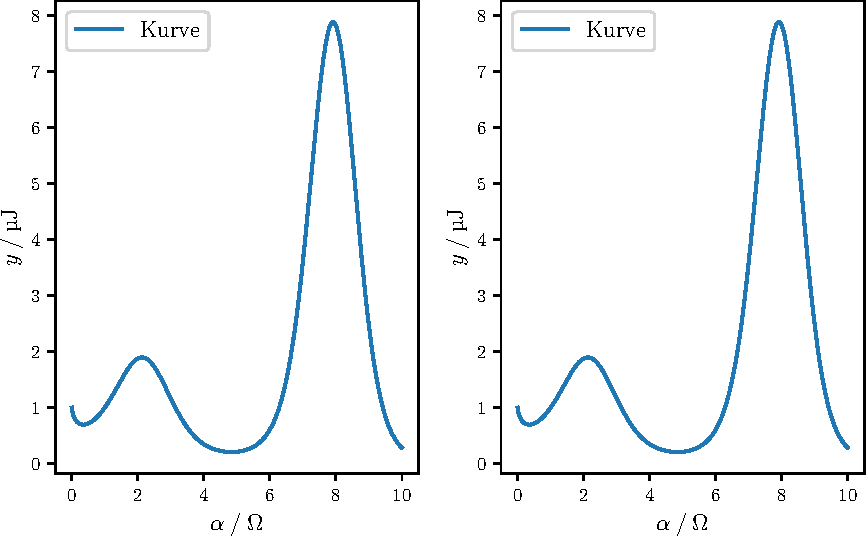
\includegraphics[width=0.75\textwidth]{build/plot.pdf}
  \caption{Filterkurve des Selektivverstärkers.}
  \label{fig:plot}
\end{figure}

\noindent
Aufgrund von hohen Schwankungen der Geräte, auf die in der Diskussion (\autoref{sec:Diskussion}) näher eingegangen wird, wurde für den weiteren Verlauf eine Frequenz von $\SI{35}{\kilo\hertz}$ verwendet.
Die Kenngrößen der Brückenschaltung sind in \autoref{tab:kennGrBr} dargestellt. 
\begin{table}[H]
  \centering
  \caption{Kenngrößen der Brückenschaltung.}
  \label{tab:kennGrBr}
  \begin{tabular}{c | c}
    \toprule
    Kenngröße & Wert \\
    \midrule
    Frequenz $\nu$ & $\SI{35}{\kilo\hertz}$ \\
    Speisespannung $U_{\text{Sp}}$ & $\SI{1}{\volt}$ \\
    Windungszahl $n$ & 250 \\
    Querschnitt der Spule $F$ & $\SI{86,6}{\square\milli\meter}$ \\
    Spulenlänge $L$ & $\SI{13,5}{\centi\meter}$ \\
    \bottomrule
  \end{tabular}
\end{table}

\noindent
In dem Versuch wurde keine Verstärkung in der Schaltung verwendet, weshalb auch keine eingerechnet werden muss.
Die Messwerte sind in insgesamt vier Tabellen aufgeteilt. In \autoref{tab:NdMessw} sind die Messwerte für Neodym, in \autoref{tab:GdMessw} die Werte für Gadolinium und in \autoref{tab:DyMessw} die Daten für Dysprosium aufgelistet.
Es ist darauf zu achten, dass der Lufteinschluss in der Probe, die eine Länge von $\SI{0,8}{\centi\meter}$ hat, bereits aus der Länge der Probe herausgerechnet wurde.
\begin{table}[H]
  \centering
  \caption{Messwerte der Widerstände und Spannungen der Brückenschaltung bei $\SI{35}{\kilo\hertz}$ und $\SI{60}{\milli\volt}$ bei Neodym.}
  \label{tab:NdMessw}
  \begin{tabular}{c| c c c c}
    \toprule
    Durchlauf & $R_3 \,/\, \si{\ohm}$ & $R_4 \,/\, \si{\ohm}$ & $\upDelta R \,/\, \si{\ohm}$ & $U_{\text{Br}} \,/\, \si{\milli\volt}$ \\%Welche Brückenspannung ist hier gefragt? Ich bin von der Ausgegangen, die am Voltmeter angezeigt wird, wenn die Probe eingesteckt wird
    \midrule
    Erster & 0,925 & 4,075 & 0,175 & 49 \\
    Zweiter & 0,925 & 4,075 & 0,200 & 49 \\
    Dritter & 0,925 & 4,075 & 0,190 & 49 \\
    Mittelwerte & 0,925 & 4,075 & 0,188 & 49\\
    \bottomrule
  \end{tabular}
\end{table}

\begin{table}[H]
  \centering
  \caption{Messwerte der Widerstände und Spannungen der Brückenschaltung bei $\SI{35}{\kilo\hertz}$ und $\SI{60}{\milli\volt}$ bei Gadolinium.}
  \label{tab:GdMessw}
  \begin{tabular}{c| c c c c}
    \toprule
    Durchlauf & $R_3 \,/\, \si{\ohm}$ & $R_4 \,/\, \si{\ohm}$ & $\upDelta R \,/\, \si{\ohm}$ & $U_{\text{Br}} \,/\, \si{\milli\volt}$ \\
    \midrule
    Erster & 0,925 & 4,075 & 0,90 & 67,0 \\
    Zweiter & 0,925 & 4,075 & 0,90 & 69,0 \\
    Dritter & 0,925 & 4,075 & 0,80 & 69,0 \\
    Mittelwerte & 0,925 & 4,075 & 0,87 & 68,3\\
    \bottomrule
  \end{tabular}
\end{table}

\begin{table}[H]
  \centering
  \caption{Messwerte der Widerstände und Spannungen der Brückenschaltung bei $\SI{35}{\kilo\hertz}$ und $\SI{60}{\milli\volt}$ bei Dysprosium.}
  \label{tab:DyMessw}
  \begin{tabular}{c| c c c c}
    \toprule
    Durchlauf & $R_3 \,/\, \si{\ohm}$ & $R_4 \,/\, \si{\ohm}$ & $\upDelta R \,/\, \si{\ohm}$ & $U_{\text{Br}} \,/\, \si{\milli\volt}$ \\
    \midrule
    Erster & 0,925 & 4,075 & 1,675 & 30,75 \\
    Zweiter & 0,925 & 4,075 & 1,675 & 30,75 \\
    Dritter & 0,925 & 4,075 & 1,675 & 30,75 \\
    Mittelwerte & 0,925 & 4,075 & 1,675 & 30,75 \\
    \bottomrule
  \end{tabular}
\end{table}

\noindent
Die \autoref{tab:alleMessw} zeigt alle Mittelwerte übersichtlich auf einen Blick. Zudem sind die Messwerte für einen Durchlauf ohne Füllung zu entnehmen.
Es ist dabei darauf zu achten, dass für die Messung der Dysprosiumfüllung das Millivoltmeter umskaliert wurde, weshalb die Brückenschaltung noch ein zweites Mal ohne eine Probe vermessen werden musste.
Zu den beiden verstellbaren Widerständen kommen noch die $\SI{998}{\ohm}$ der vor und nach des Potentiometers geschalteten Widerstände hinzu.
\begin{table}[H]
  \centering
  \caption{Mittlere Messwerte der Widerstände und Spannungen der Brückenschaltung bei $\SI{35}{\kilo\hertz}$ und $\SI{60}{\milli\volt}$ in Abhängigkeit der Spulenfüllung.}
  \label{tab:alleMessw}
  \begin{tabular}{c| c c c c}
    \toprule
    Füllung & $\overline{R_3} \,/\, \si{\ohm}$ & $\overline{R_4} \,/\, \si{\ohm}$ & $\overline{\upDelta R} \,/\, \si{\ohm}$ & $\overline{U_{\text{Br}}} \,/\, \si{\milli\volt}$ \\
    \midrule
    ohne Probe & 998,925 & 1002,08 & 0,900 & 67,00 \\
    Neodym & 998,925 & 1002,08 & 0,188 & 49,00\\ 
    Gadolinium & 998,925 & 1002,08 & 0,870 & 68,30\\ \hline
    ohne Probe & 998,925 & 1002,08 & 0,900 & 13,50 \\
    Dysprosium & 998,925 & 1002,08 & 1,675 & 30,75 \\
    \bottomrule
  \end{tabular}
\end{table}

\noindent
Die Suszeptibilität wird über zwei verschiedene Wege berechnet. Die erste Suszeptibilität $\chi_1$ wird über die Gleichung (\ref{eqn:susz1}) berechnet, die zweite $\chi_2$ mithilfe von Gleichung (\ref{eqn:susz2}).
Die Querschnittsfläche $Q$ durch die effektive Querschnittsfläche $Q_{\text{eff}}$
\begin{align*}
  Q_{\text{eff}} = Q\frac{\rho}{\rho_w} = \frac{m}{L\cdot\rho_w}
\end{align*}
ersetzt. Dabei ist $\rho$ die Dichte des Pulvers, $\rho_w$ die Dichte eines Einkristalles, $m$ die Masse des Pulvers und $L$ die Länge der Probe.
Die daraus resultierenden Werte sind in \autoref{tab:SuszWerte} mit der Masse $m$ und der Einkristalldichte $\rho_w$ der Proben tabelliert.
\begin{table}[H]
  \centering
  \caption{Experimentell bestimmte Suszeptibilitäten und die zu den Proben gehörenden Massen und Einkristalldichten.}
  \label{tab:SuszWerte}
  \begin{tabular}{c c c c c c}
    \toprule
    Stoff & $m \,/\,$ g & $\rho_w \, / \, \si{\gram\per\cubic\centi\meter}$ & $Q_{\text{eff}}$ & $\chi_1$ & $\chi_2$ \\
    \midrule
    Neodym & 18,48 & 7,24 & 0,189 & 0,037 & $0,173 \cdot 10^{-6}$  \\
    Gadolinium & 14,08 & 7,40 & 0,141 & 0,036 & $1,0691 \cdot 10^{-6}$ \\
    Dysprosium & 15,10 & 7,80 & 0,143 & 0,079 & $2,030 \cdot 10^{-6}$ \\
    \bottomrule
  \end{tabular}
\end{table}